\documentclass[12pt,a4paper]{article}
\usepackage[utf8]{inputenc}
\usepackage{graphicx}
\usepackage{geometry}
\usepackage{enumitem}
\usepackage{titlesec}
\usepackage{hyperref}

\geometry{margin=2.5cm}

\title{Registration Pattern Analysis}
\date{}

\begin{document}

\maketitle

\section*{1. Frequency of Registration Gaps (Days Between Registrations)}
As shown in Figure~\ref{fig:reg-gap}, the median gap between registrations is one day, while the mean is 35.3 days due to a few outliers. Most multi-course enrolments occur within one day, showing a clear tendency for batch registrations.

\begin{figure}[h!]
    \centering
    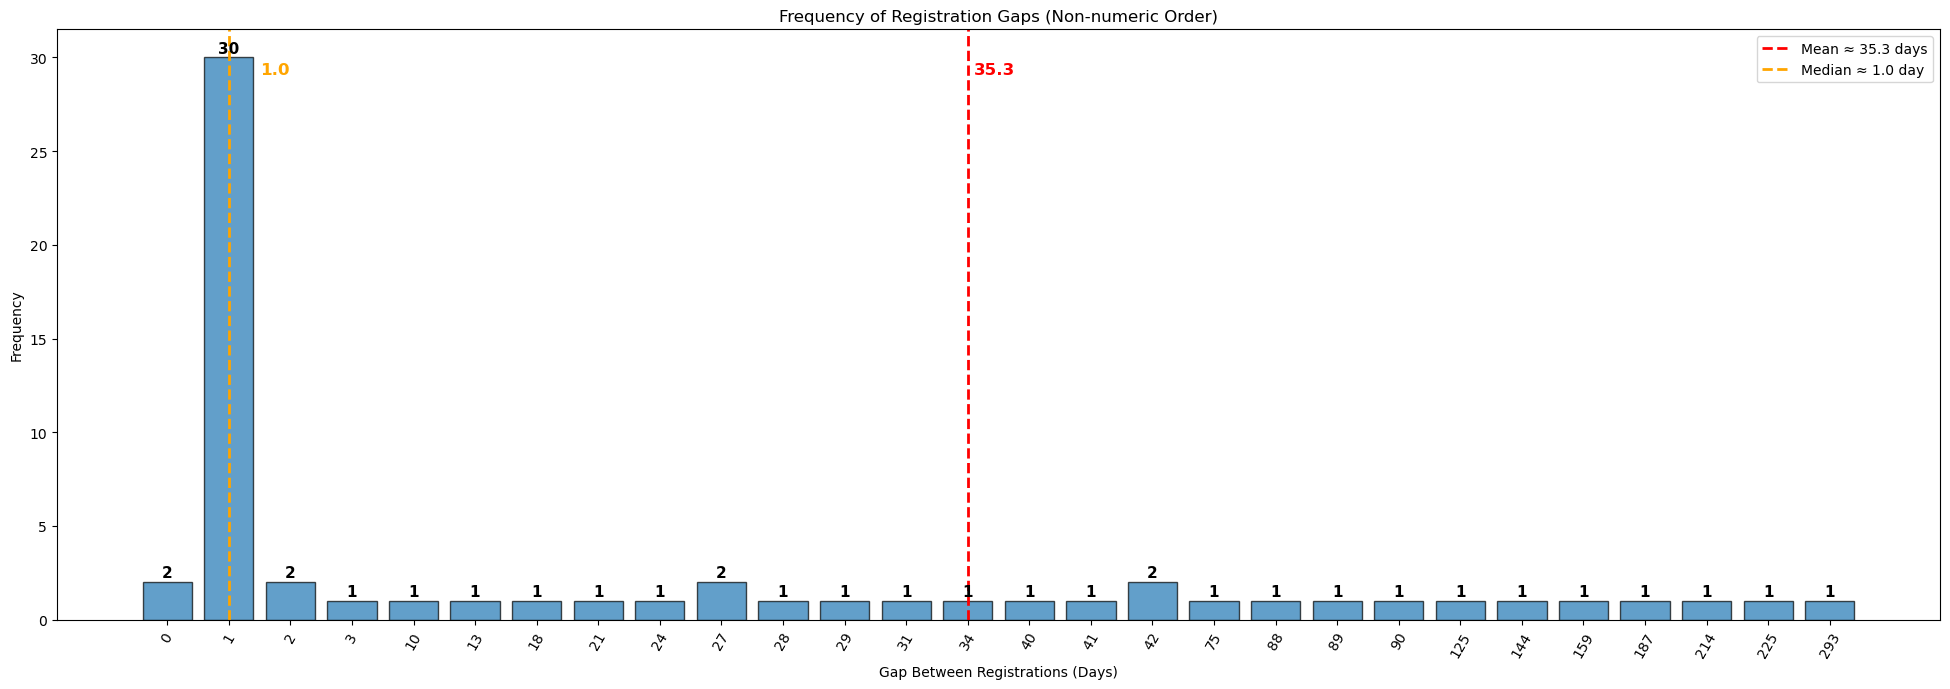
\includegraphics[width=1\textwidth]{Frequency of Registration Gaps (Days between registrations).png}
    \caption{Frequency of Registration Gaps (Days Between Registrations)}
    \label{fig:reg-gap}
\end{figure}

\section*{2. Most Popular Course Combinations in Student Baskets}
Figure~\ref{fig:combo-basket} shows that \textit{burger + pizza} is the most common bundle, followed by \textit{nugget + sausage} and other fast-food combinations.

\begin{figure}[h!]
    \centering
    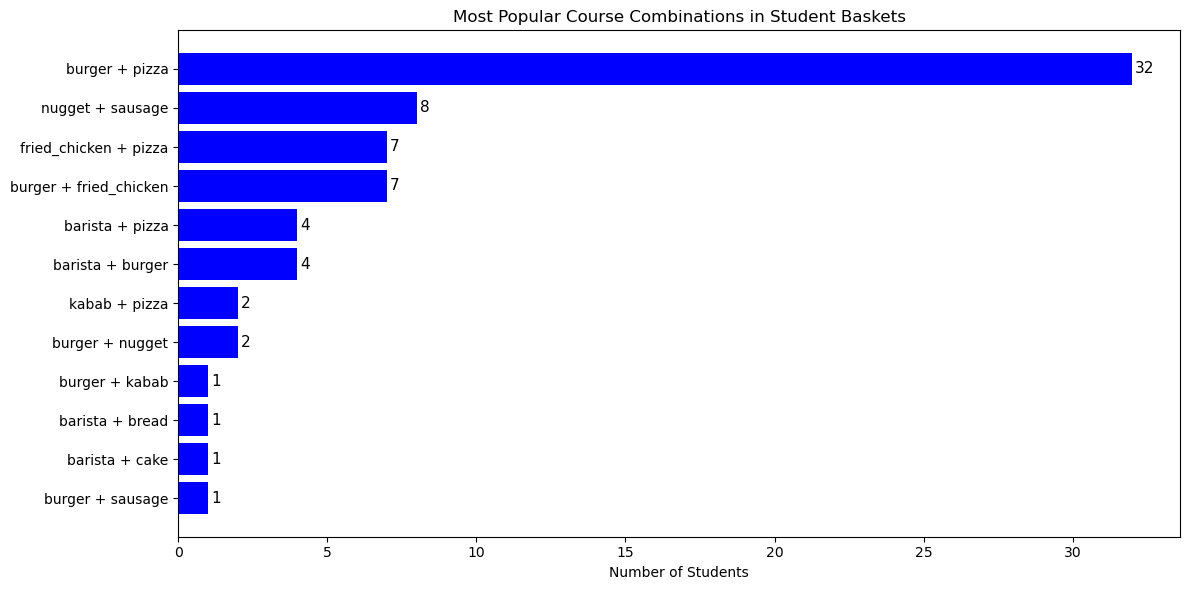
\includegraphics[width=1\textwidth]{Most Popular Course Combinations in Student Baskets.png}
    \caption{Most Popular Course Combinations in Student Baskets}
    \label{fig:combo-basket}
\end{figure}

\section*{3. Registration Sequences with 2 Courses}
Figure~\ref{fig:seq2} demonstrates that \textit{burger $\rightarrow$ pizza} is the leading sequential choice.

\begin{figure}[h!]
    \centering
    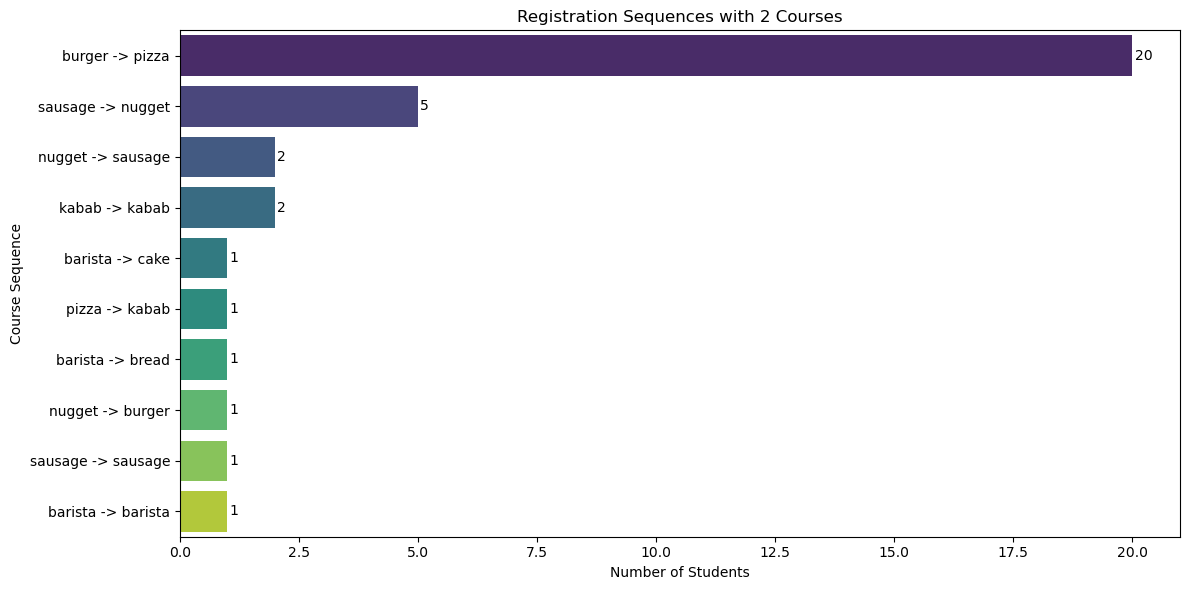
\includegraphics[width=1\textwidth]{Registration Sequences with 2 Courses.png}
    \caption{Registration Sequences with 2 Courses}
    \label{fig:seq2}
\end{figure}

\section*{4. Registration Sequences with 3 Courses}
As shown in Figure~\ref{fig:seq3}, only a handful of students follow three-step sequences, the most popular sequence being \textit{burger $\rightarrow$ pizza $\rightarrow$ fried\_chicken}.

\begin{figure}[h!]
    \centering
    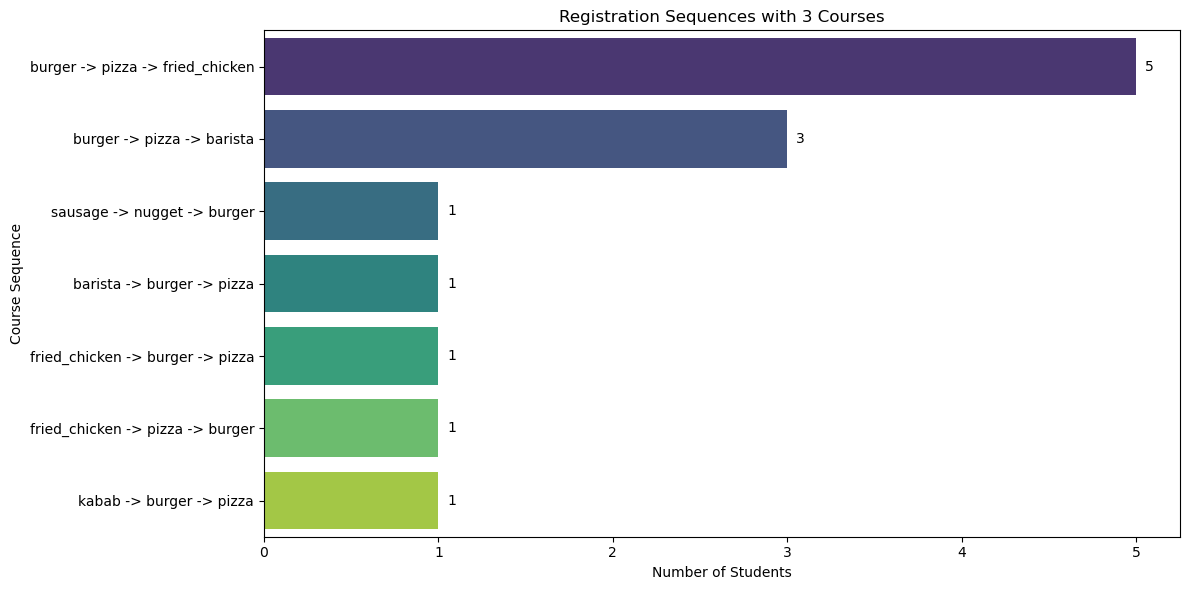
\includegraphics[width=1\textwidth]{Registration Sequences with 3 Courses.png}
    \caption{Registration Sequences with 3 Courses}
    \label{fig:seq3}
\end{figure}

\section*{5. Course Registration Network}
Figure~\ref{fig:network} displays the overall registration network, highlighting transition pathways between courses.

\begin{figure}[h!]
    \centering
    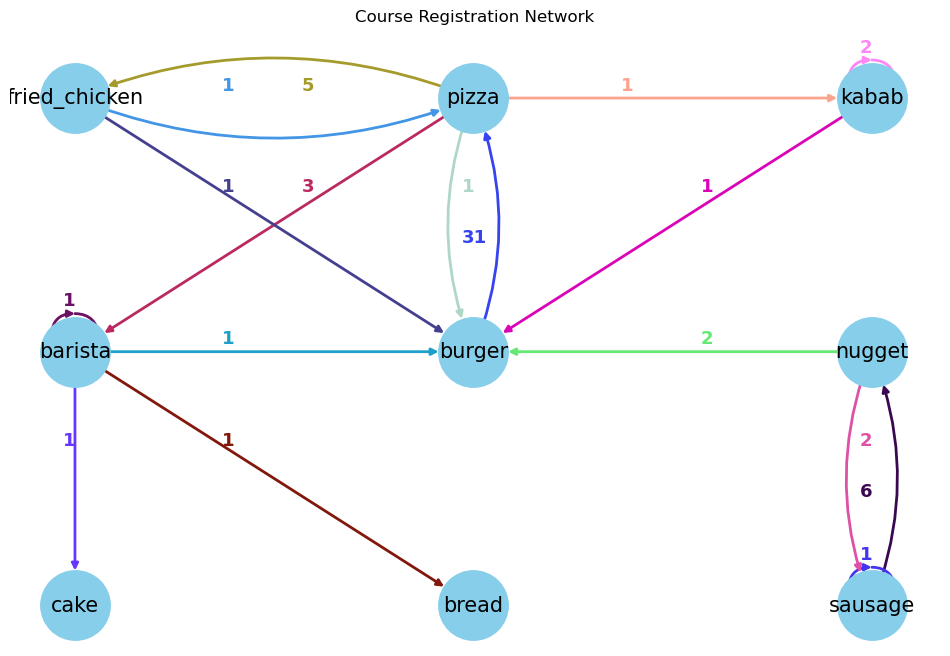
\includegraphics[width=1\textwidth]{Course Registration Network.png}
    \caption{Course Registration Network}
    \label{fig:network}
\end{figure}

\clearpage
\section*{Summary}

\begin{itemize}
    \item Most multi-course registrations happen within 1 day, showing planned or bundled registrations.
    \item Burger and pizza courses dominate both combinations and sequences.
    \item These findings are valuable for designing bundles, recommending next courses, and understanding the actual learning journey.
\end{itemize}

\end{document}